\subsection{Workshop: Workshop on Deep Learning and Inverse Problems}

Even though this workshop is dedicated to inverse problems in broad sense of this term, the majority of presentations are somehow related with imaging. 
Moreover, significant fraction of them is either dedicated to MRI reconstruction or at least somehow mention it. 
This observation underlines consensus of the research community on the importance of this problem.

\subsubsection{Uncertainty Quantification in Deep MRI
Reconstruction \cite{edupuganti2020uncertainty}}

Presented by \textit{Vineet Edupuganti}. \\

{\bf Motivation:} accelerated MRI reconstruction is unreliable, especially when generative models are applied. Need to estimate uncertainty of a reconstruction model to help radiologist to avoid mistakes. \\

{\bf Background:} most of existing approaches (Deep Ensembles \cite{Lakshminarayanan17}, VAE sampling \cite{corr/abs-2007-08128}) for epistemic uncertainty estimation leverage one or another form of the Monte Carlo sampling: several samples are utilized to compute statistics, which are then represented as results. One example of this approach is to sample from VAE and compute variance of results. However, it is impossible to compute bias without ground truth image using this method. \\

{\bf Method:} authors propose to utilize  Stein’s Unbiased Risk Estimator
(SURE) \cite{doi:10.1080/01621459.2018.1429276} to compute bias-free uncertainty estimation without reference image. For that, the following derivation is performed.

Given the ground truth image $x_0$, the zero-filled image can
be written as 

\begin{equation}
    x_{zf} = x_0 + v
\end{equation} 

where $v$ is noise. Now considering reconstruction $\hat{x}$ with
dimension $n$, one can expand test MSE as 

\begin{equation}
    \mathbb{E}|| \hat{x} - x_0 ||^2 = \mathbb{E} || x_0 - x_{zf} + x_{zf} - \hat{x} ||^2 = -n \sigma^2  + \mathbb{E} || x_{zf} - \hat{x} ||^2 + 2Cov(x_{zf}, \hat{x})
    \label{eq:sure-one}
\end{equation} 

Since $x0$ is not present in \ref{eq:sure-one}, we see that SURE serves as a surrogate for MSE even when the ground truth is unknown. 
A key assumption behind SURE is that the noise process v that relates the zero-filled image to the ground truth is normal, namely $v \sim N(0, \sigma^2
I)$. 
With this assumption SURE is formulated as follows 

\begin{equation}
    SURE = -n \sigma^2 || \hat{x} - x_zf ||^2 + \sigma^2 tr(\partial \hat{x} / \partial x_zf)
\end{equation}

\textbf{Important note:} previous assumption may not hold in practice. 

Authors show that when error in the output reconstruction is not large, and as a result $\sigma^2$ can be estimated as 

\begin{equation}
    \sigma^2 = || \hat{x} - x_{zf} ||^2  / n
\end{equation} 

This assumption allows to formulate SURE as follows 

\begin{equation}
    SURE = \sigma^2 tr(\partial \hat{x} / \partial x_zf)
\end{equation} 

\textbf{Important note:} this assumption on only holds for low acceleration rates and artefact-free reconstruction models. 
Since this method is developed for evaluation of potentially artefact-prone models, this assumption looks quite strong. \\

Further investigations are targeted on acceleration of computations of trace of the end-to-end network Jacobian, which otherwise can be problematic. 
Authors also approach the problem of the requirement for MRI noise to follow standard normal distribution. \\

{\bf Results and takeaways:} the main contribution of this work is to apply SURE to the uncertainty estimation task in the domain of medical imaging, which has not been done before. 
An example of high correlation between estimated SURE values are computed MSE error is illustrated on figure \ref{fig:sure-result}.

\begin{figure}[h!]
    \centering
    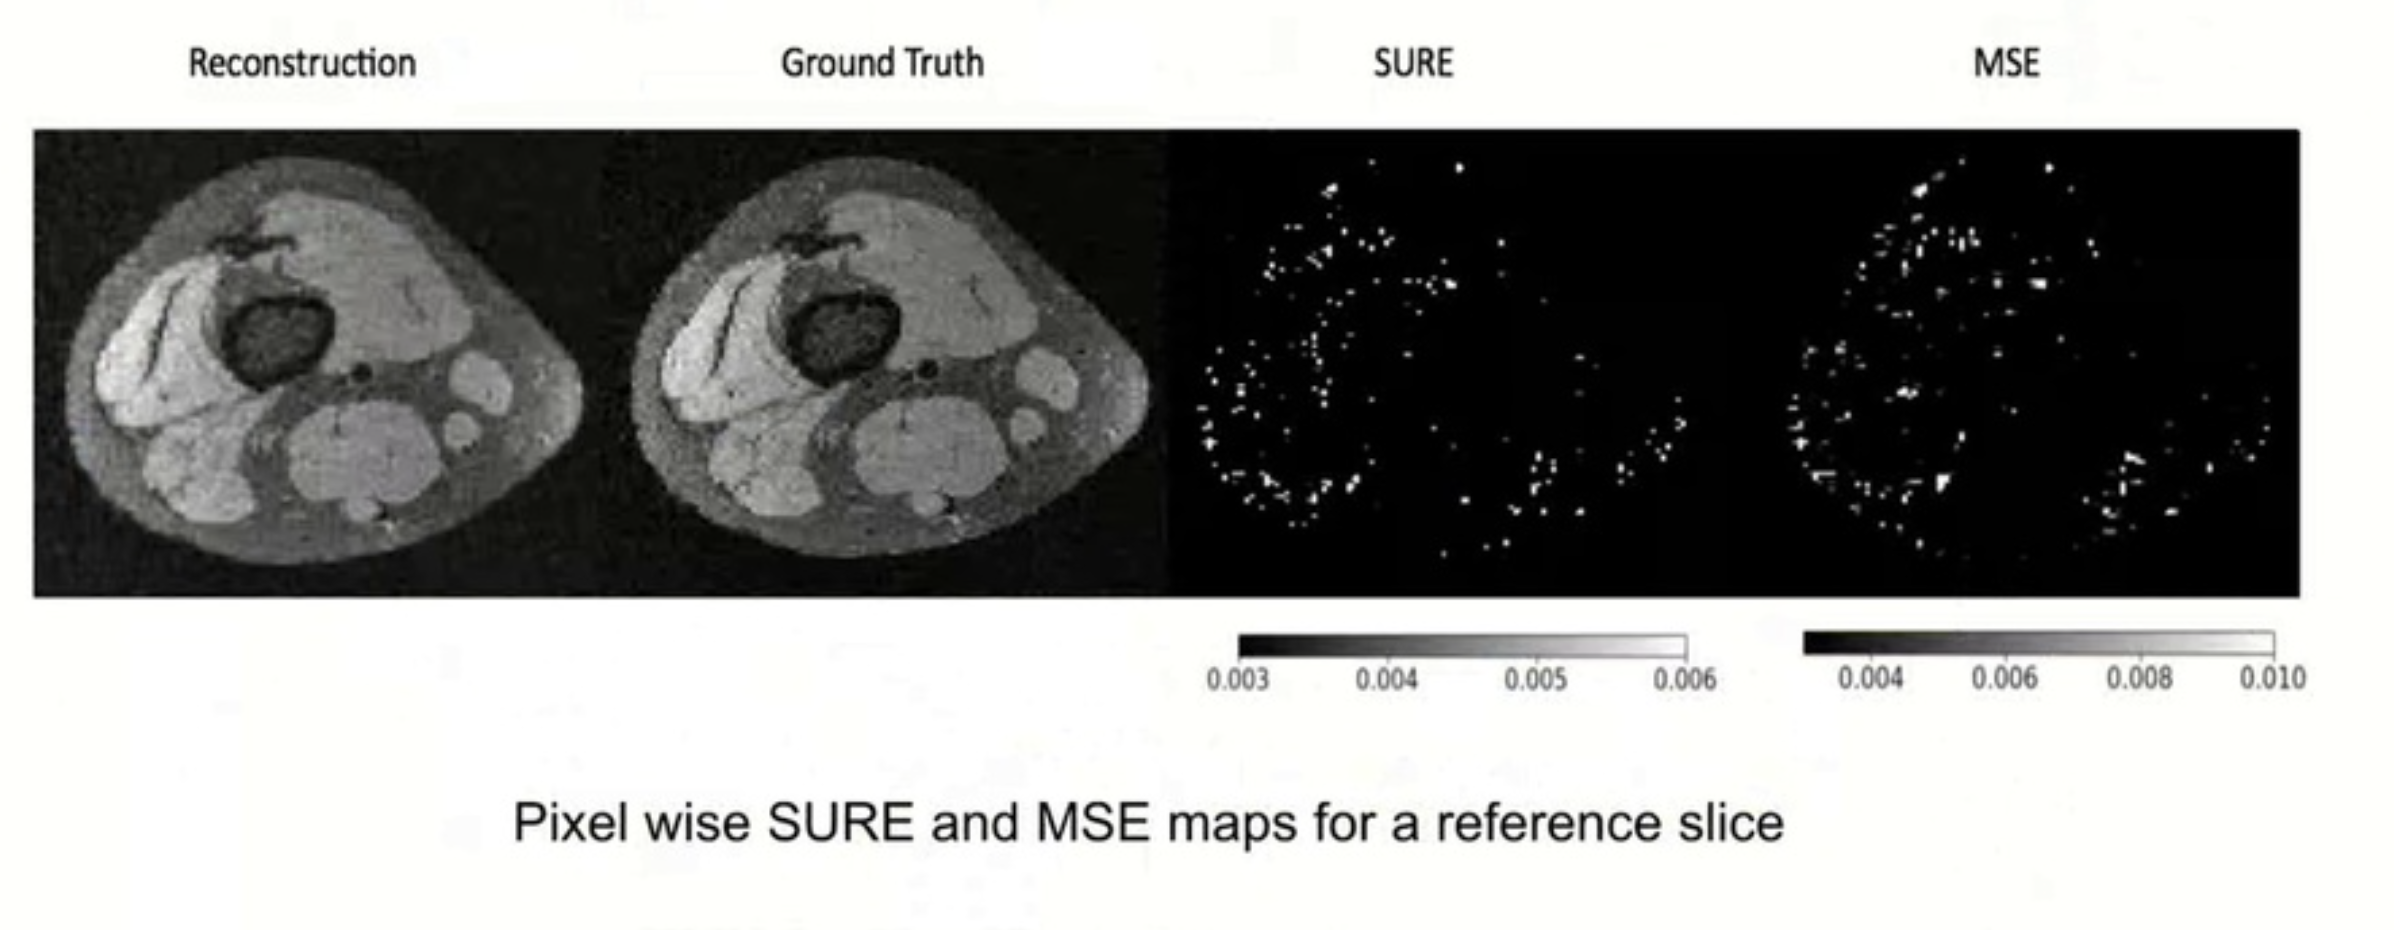
\includegraphics[scale=0.4]{neurips-2020/images/Screenshot 2020-12-12 at 17.26.28.png}
    \label{fig:sure-result}
\end{figure}





\subsubsection{Model Adaptation for Inverse Problems in Imaging \cite{gilton2020model}}

Presented by \textit{Rebecca Willett}. \\

{\bf Motivation:} having measurements $y$ and a neural network $f_{\phi}$ trained with some forward model $A_0$, make high quality reconstructions $\hat{x}$ if forward model used during inference $A_1$ is different from the one using for training ($A_0$). 
The scheme of the task setup is represented on fig. \ref{fig:inv_prob_setup}
Authors call this phenomenon a \textit{model drift}. \\

\begin{figure}[h!]
    \centering
    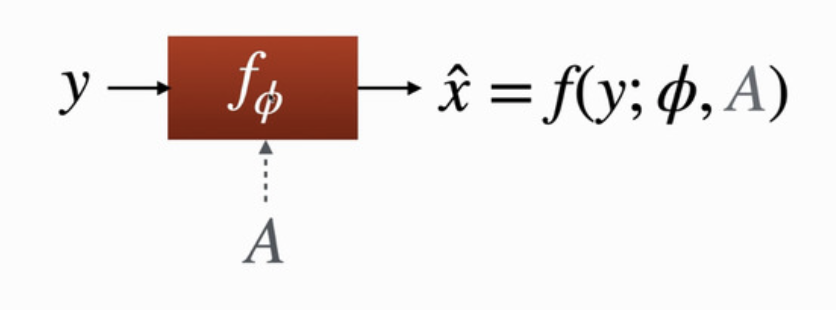
\includegraphics[scale=0.3]{neurips-2020/images/Screenshot 2020-12-13 at 20.44.08.png}
    \caption{Neural network with parameters $\phi$ (and optionally A) inputs $y$ and outputs an estimate $\hat{x}$.}
    \label{fig:inv_prob_setup}
\end{figure} 

{\bf Example:} train a fast MRI network with one acceleration rate but perform inference on some different acceleration rate. 
Even if the acceleration rate is lower, there is a domain shift that makes the network less capable to produce a high-quality estimate. \\

{\bf Definitions:} 
\begin{itemize}
    \item {\bf Distribution drift:} $p(X, Y)$ changes \textit{in unknown way} between train and deployment
    \item {\bf Model drift:} $p(X, Y)$ changes \textit{in known or partially known way} between train and deployment
    \item {\bf Domain adaptation:} first train with many samples $(x_i^{(0)}, y_i^{(0)}) \sim p_0$, then adapt using few samples from $(x_i^{(1)}, y_i^{(1)}) \sim p_1$
    \item {\bf Model adaptation:} first train with many samples $(x_i^{(0)}, y_i^{(0)}) \sim p_0$ and, then adapt using few samples from  $(?, y_i^{(1)}) \sim p_1$ (images are not known) 
\end{itemize}
\\ 

{\bf Method:} train a reconstruction network for a known forward model then adapt to a new forward model without access to ground truth images, and without knowing the exact parameters of the new forward model. \\

\underline{Proposed approaches are:}   

{\bf Parametrize and Perturb}: use calibration data to \textit{perturb} parameters of the original reconstruction network. 
In practice it means conversion of $f_0$ to some $f_1$ that will be able to handle $A_1$.

\begin{figure}[h!]
    \centering
    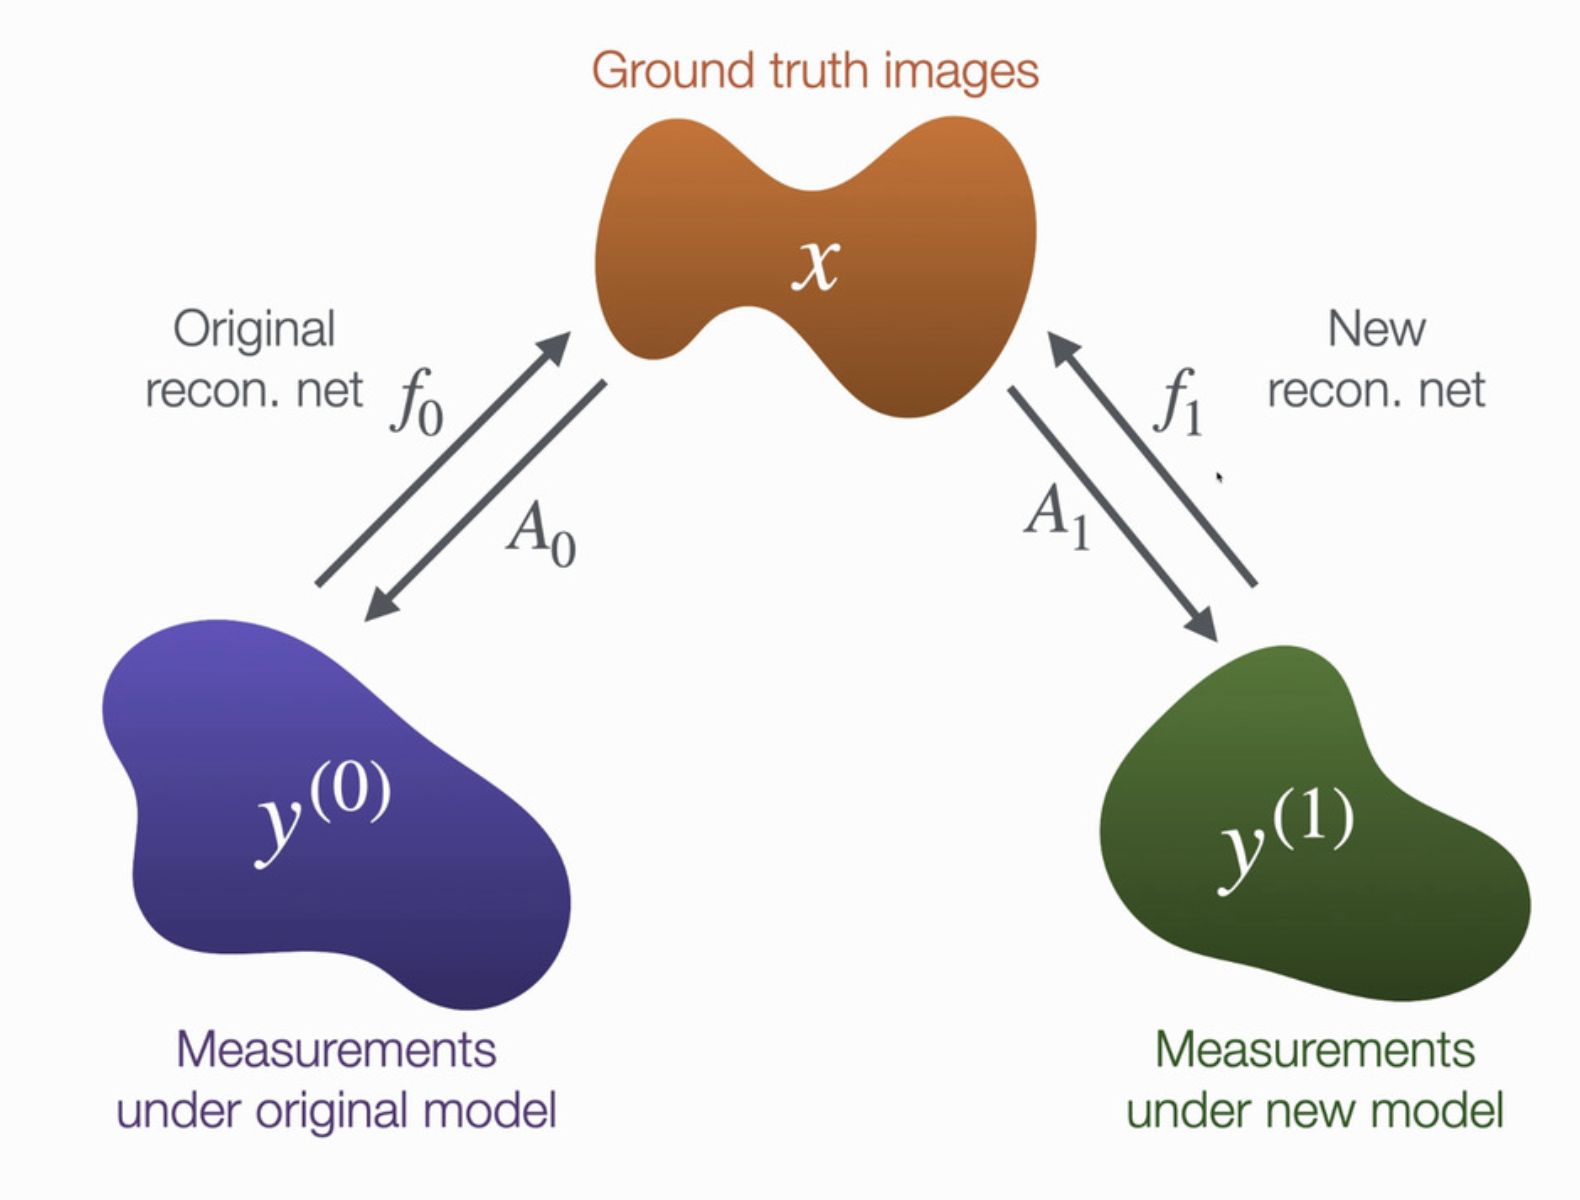
\includegraphics[scale=0.4]{neurips-2020/images/Screenshot 2020-12-13 at 21.21.21.png}
    \caption{Illustration of the Parametrize and Perturb approach. $f$ is perturbed to be able to handle $A_1$ during the inference time.}
    \label{fig:PP_approach}
\end{figure} \\

{\bf Condition and Correct}: train a new (correction) network $h_{\theta}$ to map $A_1$ to $A_0$ and then apply $f_{\phi}$.

\begin{figure}[h!]
    \centering
    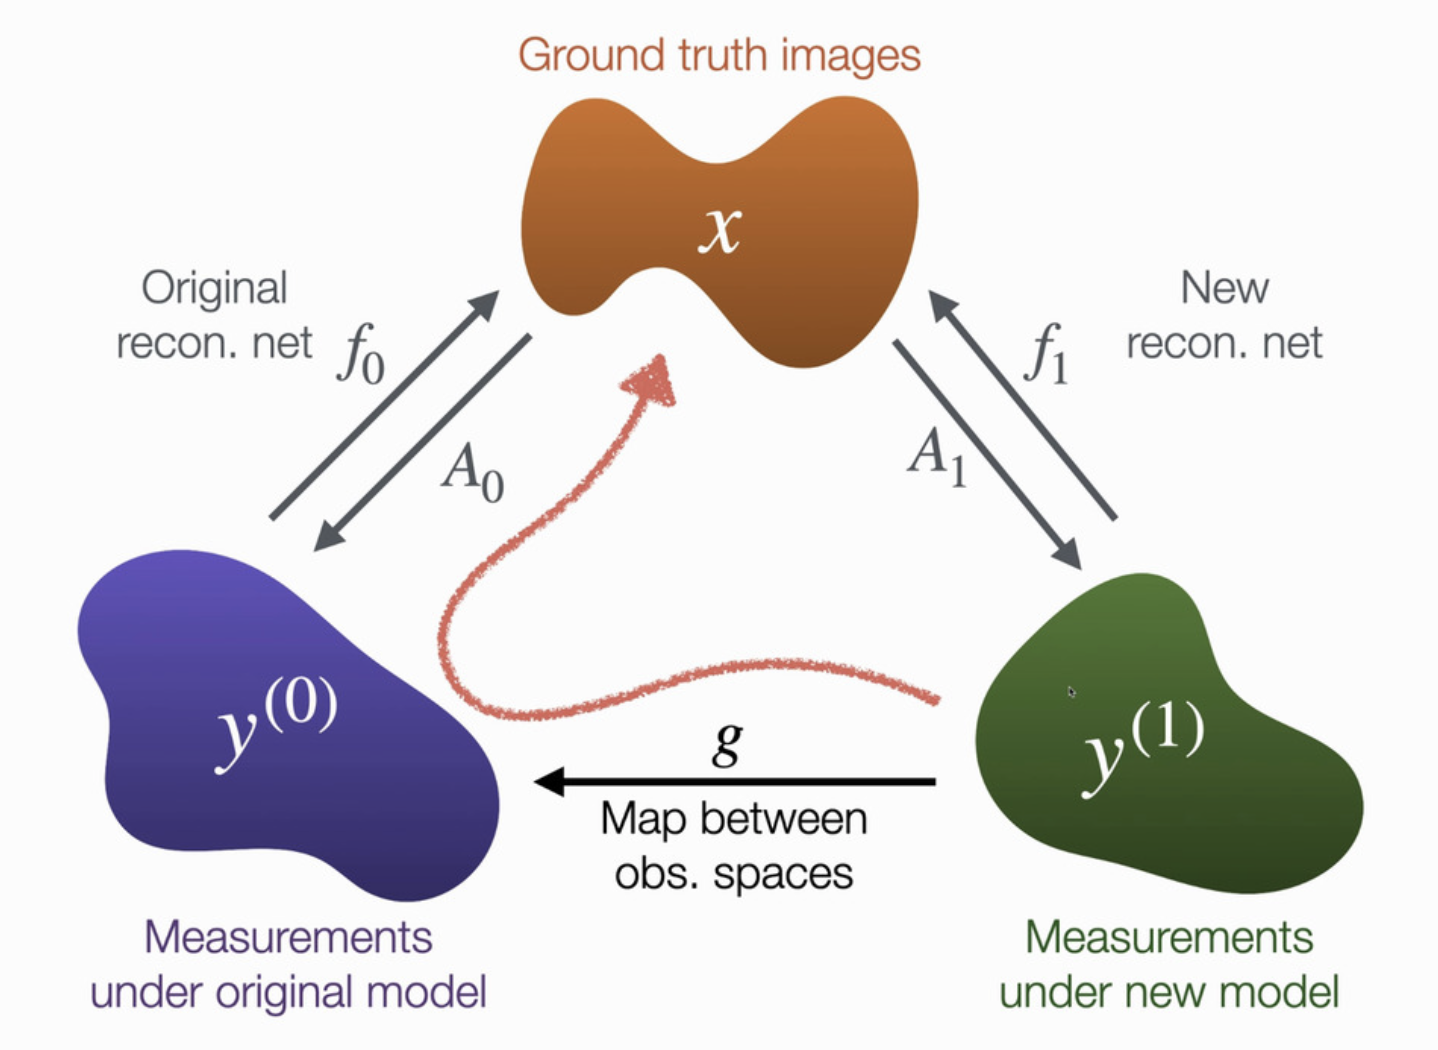
\includegraphics[scale=0.4]{neurips-2020/images/Screenshot 2020-12-13 at 21.24.26.png}
    \caption{Illustration of the Condition and Correct approach. Output of the $A_1$ is made similar to $A_0$ and then $f_\phi$ is applied}.
    \label{fig:my_label}
\end{figure}



{\bf Results:} authors show high-quality results (fig. \ref{fig:adaptation_results_11}, \ref{fig:adaptation_results_2}, \ref{fig:fast_mri_recon}, \ref{fig:moco_recon}), which confirm that their methods allow to increase the quality of resulting images if model drift takes place.
More concretely:
\begin{itemize}
    \item Condition and Correct method, in general, works a little bit better.
    \item The most significant visual improvements are presented for the motion correction problem.
    \label{fig:adaptation_results_11}
\end{itemize}

\begin{figure}[h!]
    \centering
    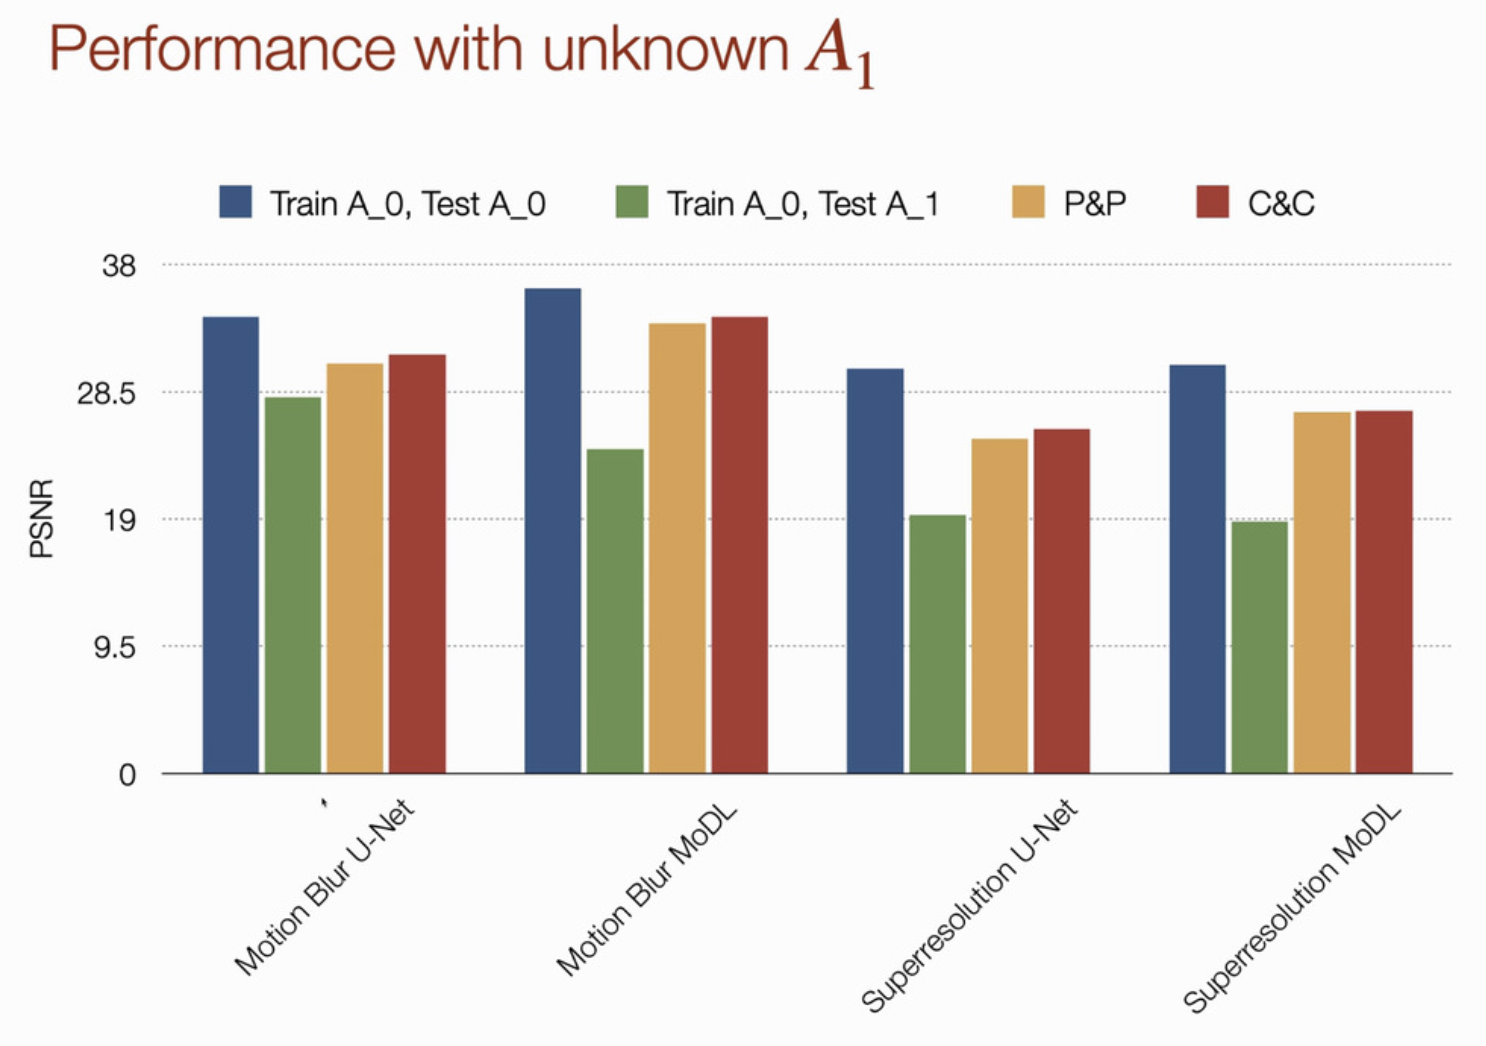
\includegraphics[scale=0.4]{neurips-2020/images/Screenshot 2020-12-13 at 21.34.45.png}
    \caption{Comparison between performance of the reconstruction model in case if $A_1$ is unknown (realistic setting) on various inverse problems.}
    \label{fig:adaptation_results_2}
\end{figure}

\begin{figure}[h!]
    \centering
    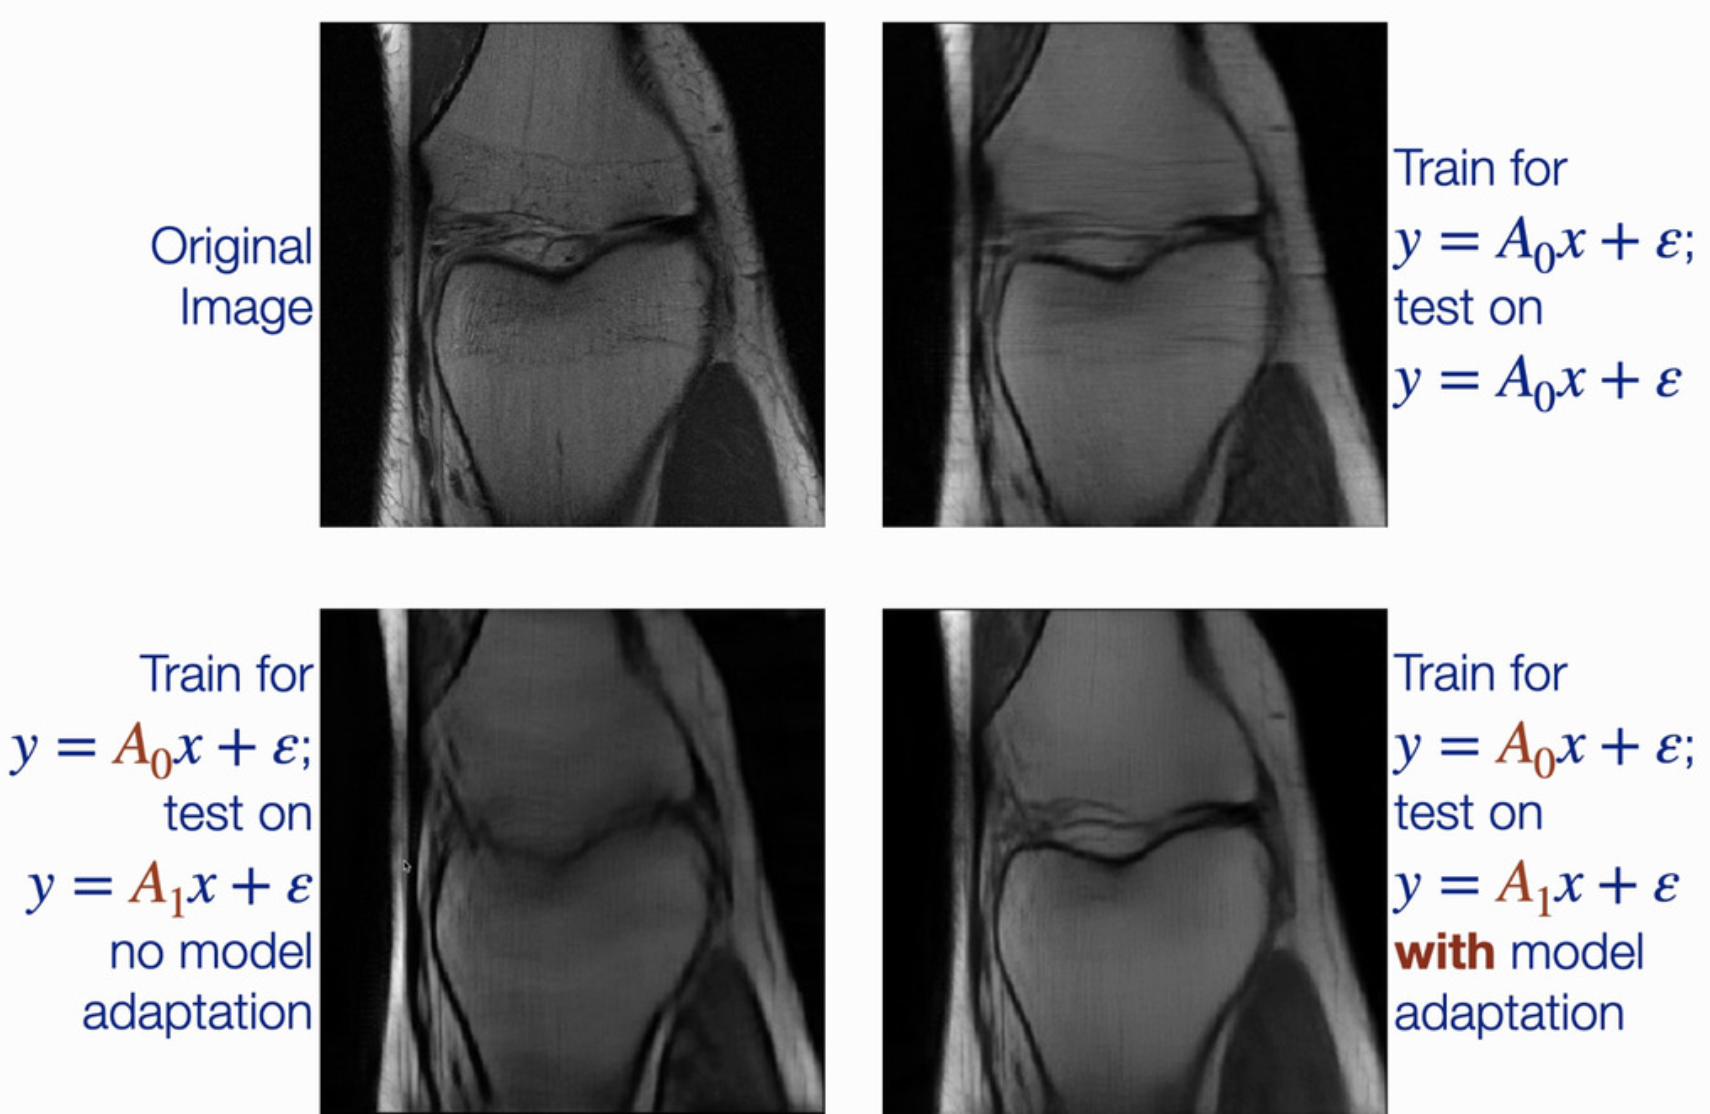
\includegraphics[scale=0.4]{neurips-2020/images/Screenshot 2020-12-13 at 21.13.23.png}
    \caption{Example of the performance of the proposed method for the fast MRI reconstruction problem}
    \label{fig:fast_mri_recon}
\end{figure}

\begin{figure}[h!]
    \centering
    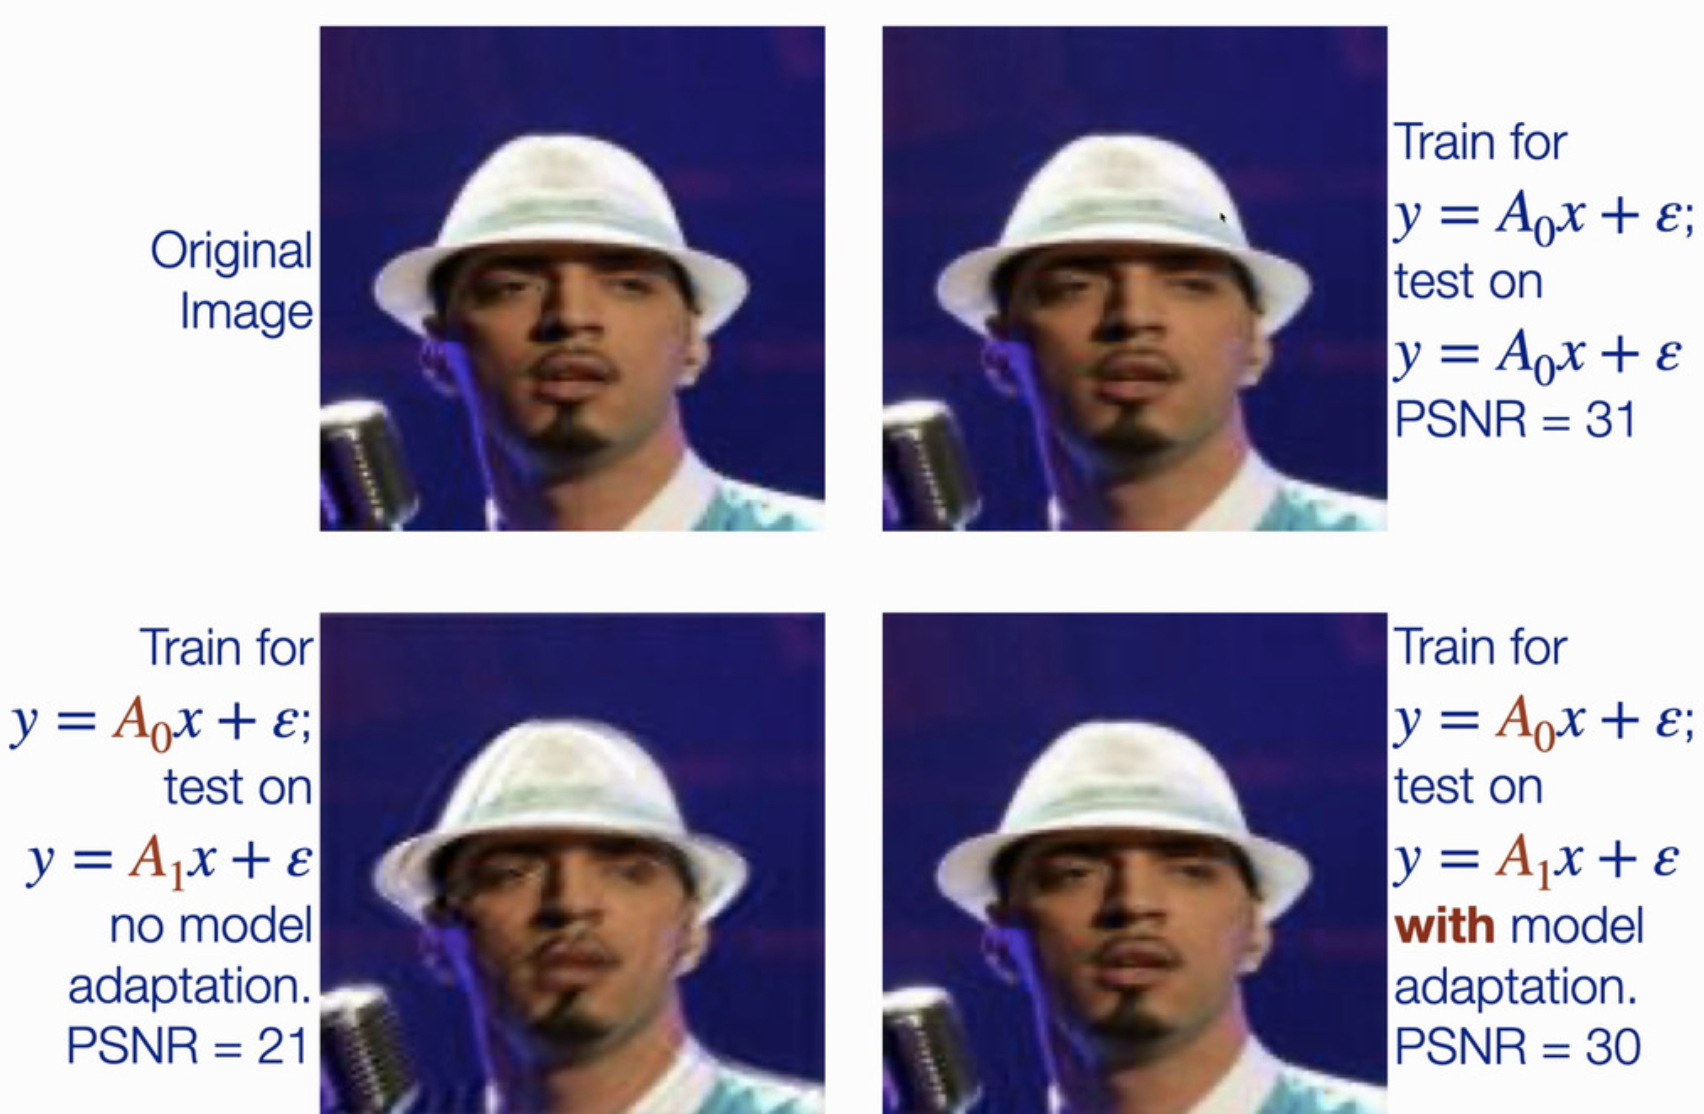
\includegraphics[scale=0.4]{neurips-2020/images/Screenshot 2020-12-13 at 21.13.52.png}
    \caption{Example of the performance of the proposed method for the general domain motion correction problem}
    \label{fig:moco_recon}
\end{figure}





\subsubsection{fastMRI}

Presented by \textit{Larry Zitnick}. \\

{\bf Motivation:} describe the fastmMRI problem, present a network by organizers of the fastMRI challenge, describe model evaluation process \\

{\bf Note:} for some reason problem of the fastMRI challenge 2019 are discussed. 
Not sure why authors did not also include discussion of this year's problem. \\

{\bf Problem:} reconstructions from the model have less noise hence look unnatural to radiologists.

{\bf Solution:} add noise to the model recons (fig. \ref{fig:smooth_fastmri}). 
This approach worked good for them (radiologists are satisfied). \\

\begin{figure}[h!]
    \centering
    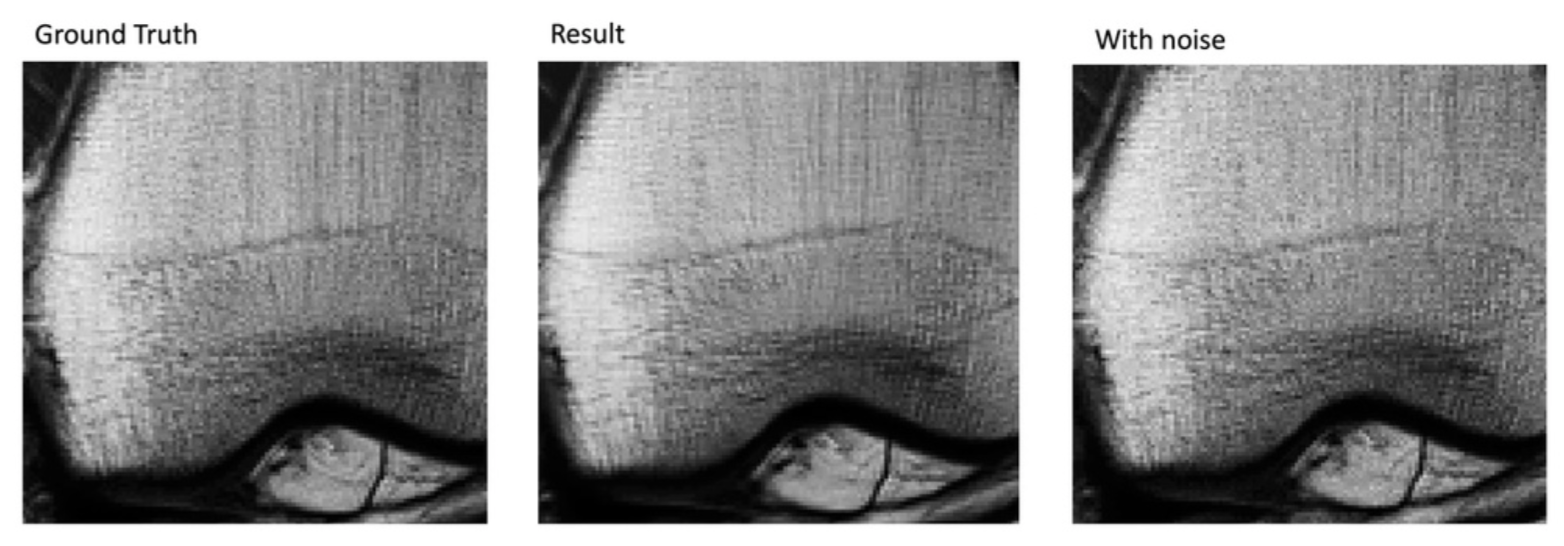
\includegraphics[scale=0.4]{neurips-2020/images/Screenshot 2020-12-13 at 22.23.29.png}
    \caption{Example of high-quality but oversmoothed result from the reconstruction model.}
    \label{fig:smooth_fastmri}
\end{figure}

{\bf Observation:} authors experienced horizontal banding artefacts (fig. \ref{fig:binding_artecats}) in their multi-coil 4x reconstructions. 
Reason - insufficient sampling pattern. 
K-space is sampled vertically (Cartesian sampling), which results in higher resolution in vertical dimension compared to the horizontal dimension and hence causing horizontal artefacts (explanation for the presenter). \\

\begin{figure}[h!]
    \centering
    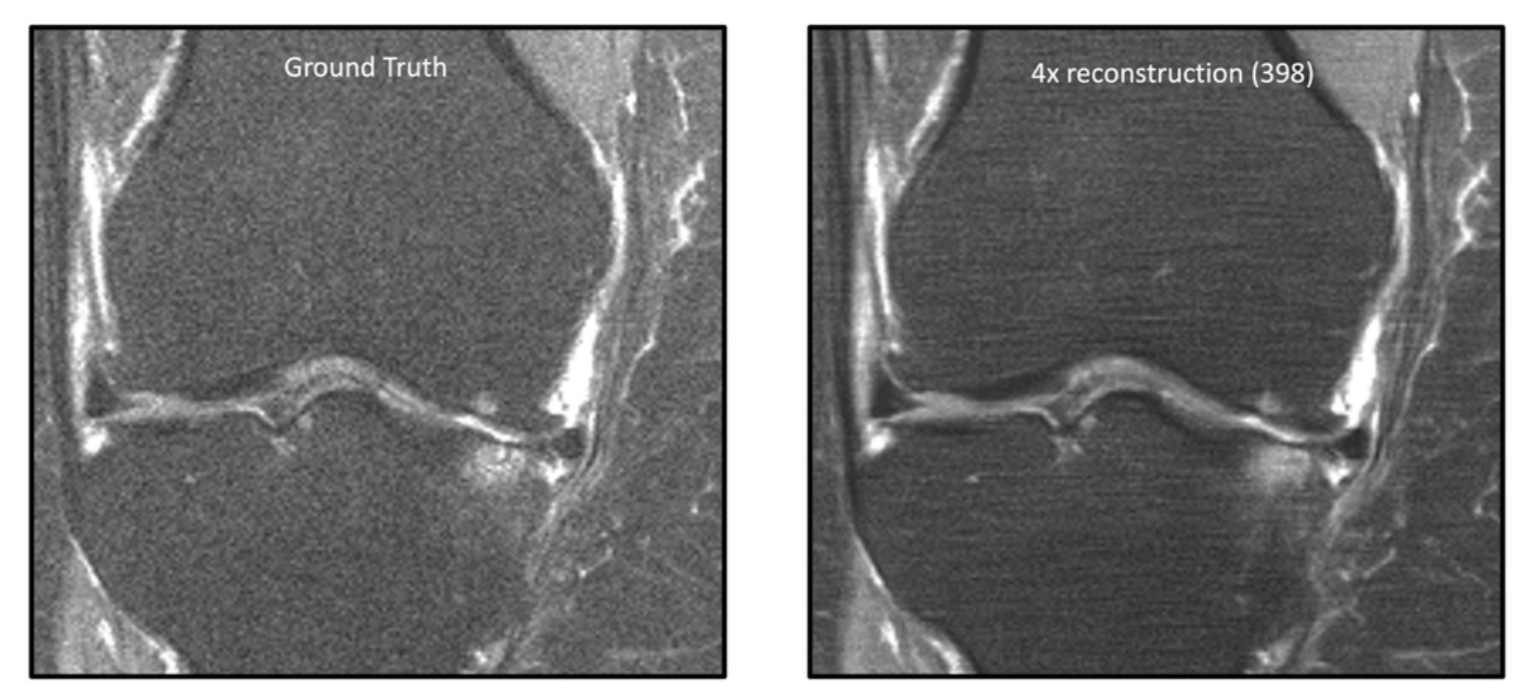
\includegraphics[scale=0.4]{neurips-2020/images/Screenshot 2020-12-13 at 22.32.40.png}
    \caption{Horizontal binding artefacts caused by insufficient sampling pattern.}
    \label{fig:binding_artecats}
\end{figure} 

{\bf Method:} most of the talk very similar to the same talk from the last year. 
The new part was the interchangeability study, which authors performed using 4x acceleration (3T) and 108 patients. 
Reconstructions were reviewed by 6 radiologists according to the following process:
\begin{itemize}
    \item Radiologist reviews a scan
    \item Waits one month
    \item Same radiologist reviews the scan
    \item Separate radiologist compares the two reports
\end{itemize} \\

{\bf Results:} in the previously described setting:
\begin{itemize}
    \item New reconstructions are diagnostically interchangeable with traditional MRIs
    \item Radiologists could not distinguish which images were produced with AI and which came from the slower traditional scans
    \item All examiners rated the AI-generated images as being higher in quality than traditional scans
\end{itemize}

Note that all these results are obtained only for a single anatomy (knee) and for a limited number of protocols (only the ones that are present in the fastMRI knee dataset).







